\documentclass[12pt]{article}
\usepackage[utf8]{inputenc}
\usepackage{booktabs}
\usepackage{multirow}
\usepackage{rotating}
\usepackage{bigstrut}

%% fonts
\usepackage[utopia]{mathdesign}
\usepackage[scaled=.95]{inconsolata}

%% page margins, inter-paragraph space and no chapters
\usepackage[margin=1.1in]{geometry}
\setlength{\parskip}{0.5em}
\renewcommand{\thesection}{\arabic{section}}

%% bibliography
%\usepackage[american]{babel}
%\usepackage{csquotes}
%\usepackage[style=apa,natbib=true,backend=biber]{biblatex}
%\DeclareLanguageMapping{american}{american-apa}
%\addbibresource{EITC.bib}

%% For actual bib
\usepackage{natbib}
\bibpunct{(}{)}{,}{author-year}{}{,}

%% Fuck with the title
\makeatletter
\renewcommand{\maketitle}{\bgroup\setlength{\parindent}{0pt}
\begin{flushleft}
  \textbf{\@title}

  \@author
\end{flushleft}\egroup
}
\makeatother

%% for memisc
\usepackage{booktabs}
\usepackage{dcolumn}

%% define a dark blue
\usepackage{color}
\definecolor{darkblue}{rgb}{0,0,.5}

%% hyperlinks to references
\usepackage{hyperref}
\hypersetup{colorlinks=true, linkcolor=darkblue, citecolor=darkblue, filecolor=darkblue, urlcolor=darkblue}

\author{Adam Olson\\University of Minnesota\\February 9, 2014}
\title{Literature Review Draft}
\date{February 9, 2014}

\begin{document}
\maketitle

\section{Introduction}
Traditionally, many scholars who study comparative welfare states refer to the United States as exceptional because they believe any welfare state the United States had was less generous, developed later, and was smaller than welfare states in comparable developed countries (See especially \citealt{andersen1990}). In a very well received challenge to this conventional wisdom, \citet{hacker2002} pointed out, the ``welfare state'' is a contested idea both among political activists and scholars of welfare politics and that not every country provides social policy in a uniform manner. Since then, scholars including Jacob Hacker, Christopher Howard, and others have made a compelling case that the United States is \emph{not} smaller or less generous than European welfare states, but instead have argued that what ``is exceptional about the American welfare state is not the level of spending but the source'' of spending \citep[pg. 7]{hacker2002}.

To that point, social policy in the the United States generally belongs to one of two types: visible welfare programs and hidden welfare programs. Visible welfare programs are what most people view as welfare programs in the United States such as Medicare or Social Security. These are programs that are generally well known to politicians, interest groups, and the mass public and they are consistently salient in the national agenda. Traditionally, these are the programs which scholars refer to when they discuss measurements such as welfare effort or welfare spending - they are apparent attempts by the government to alleviate some socially undesirable problem such as poverty or hunger.

Hidden welfare programs, also known as the hidden welfare state, at the most basic level is social policy that is distributed through the tax code as tax expenditures \citep{howard1997}\footnote{A more legalistic definition of tax expenditures is provided in the the Congressional Budget and Impoundment Control Act of 1974 as ``revenue losses attributable to provisions of the Federal tax laws which allow a special exclusion, exemption, or deduction from gross income or which provide a special credit, a preferential rate of tax, or a deferral of tax liability.''}.  This type of welfare through the tax code cost the federal government 1.1 trillion dollars in 2013 which by some estimates is more than was spent on visible welfare programs \citep{omb2013}. Whereas, elderly Americans can apply for social security once they turn 62, then receive a check each month, the hidden welfare state is largely administered through the tax code without much bureaucratic overhead like with Social Security. Like in the visible welfare state, the government tries to alleviate social ills such as poverty or hunger, but it does so in a way that is not evident to most people and generally uses less obvious policy making processes \citep{mettler2011}.

While our understanding of the hidden welfare state and thus the political aspects of American social policy has increased overall due to the recent work on the hidden welfare state, it remains incomplete.  Specifically, there remain three sizable gaps in the literature. First, previous literature has studied hidden welfare programs largely in isolation from visible programs. This necessarily produces an incomplete story in trying to understand the politics of American social policy on a broader level. Both visible and hidden programs seek to alleviate some sort of social ill and while the programs utilize different strategies to accomplish this goal, they remain linked together by this common goal. For example, the United States has several ways it tries to provide housing. Home owners can deduct large parts of their mortgage from their federal income tax, they also provide vouchers to help subsidize rent, and in some cases even provide housing itself. How did America develop a housing policy which incorporates both hidden and visible spending? By examining both hidden and visible programs that have similar goals we can understand how the politics of hidden policies are both similar and different from visible programs in such a way that increases our understanding of American social policy creation and development.

The second gap deals with the idea that policy creation involves both a creation component \emph{and also} a persistence component. Policy is both the conclusion of one process and the start of another. After a policy is created, it has the potential to be expanded or retrenched by enterprising members of Congress (MCs). A policy that was created fifty years ago may look nothing like it looks today because of subsequent reforms. This overlaps with the first problem of not considering visible and hidden policies together as a visible policy may be retrenched even while a very similar hidden policy is expanded. Historically there has been attention paid to an individual policy's entire life, including after initial passage (see especially \cite{derthick1979, hacker2002}), but most of the theories seeking to explain how the United States developed the welfare state that it did, are only concerned with initial policy creation. 

The third major gap in this type of policy making literature is that there is a lack of emphasis on the role congressional behavior and institutions play in policy making. The role of Congress in creating social policy is preeminent yet literature on how the United States creates welfare policy is strangely devoid of insight from the extremely voluminous literature on congressional policy making. We have tremendous insight as to the role congressional parties, divided government, congressional committees, and many other facets of congressional life have on the behavior of individual MCs and Congress as a whole. While Congress often plays a staring role in scholarly accounts of social policy creation, this research seldom formally incorporates the scholarly insight produced by congressional scholars. By applying some of the specific hypotheses outlined by congressional scholars to the historical creation and subsequent development of the American welfare state, we will be able to see how different congressional politics create different policy outcomes.

Broadly, this dissertation asks how the United States came to rely on a mix of visible and hidden policies to provide social policy. In pursuing that question, I will draw heavily on the congressional institutions and behavior literature in formulating casual hypotheses. Additionally, it will answer why a legislator chooses to use one form of welfare policy over another to advance their goals. Consequently, this dissertation will be able to examine how individual programs are created \emph{and} persist vis-a-vie each other. The juxtaposition of the traditional American welfare state literature, hidden welfare state literature, and also the congressional literature will drastically improve our understanding of these subjects individually but will also improve the way we view American policy making as well.  

\section{Previous Literature}

The American welfare state literature is rich and well developed, not only in descriptive accounts but also concerning relevant policy making factors. Broadly in this section, I discuss both of those parts. In the first subsection, I overview descriptively the American welfare state, focusing on the types of the mechanisms the government uses to provide social policy. In the second subsection, I describe the traditional hypotheses of social policy making in the United States and then discuss several shortcomings of these hypotheses. 

\subsection{What does American Social Policy Making Look Like?}
Many scholars have argued that social policy in the United States lags behind other developed democracies, but it is not lack of social spending that makes America unique, it is the way in which it provides social policy \citep{hacker2002}. Since the end of the second world war, the United States has predominantly used four mechanisms with which to provide social policy: visible spending, regulation, guaranteed rights, and tax expenditures \citep{pierson2007}. All of those mechanisms, but especially tax expenditures have seen explosive growth in the post war period. Tax expenditures are provisions in the tax code that favor or incentive  certain desired behavior and they are functionally equivalent to traditional government outlays or spending. In the United States tax code, there are tax expenditures for everything from buying cars and houses, to having children or working. Once tax expenditures are included in the traditional welfare effort measurement, the United States becomes average in terms of welfare spending when compared to other more `generous' nations \citep[Ch. 1]{howard2008}.

When considering the four described mechanisms of policy provision in the United States, it is important to note that these tools and their resulting policies were not created and are not maintained in isolation from one another. In fact, these tools and policies can work together, exist in conflict with one another, and layer on top of each other. Social policy in the United States seeks to alleviate a social problem. Politicians, based on the political context of the time, will utilize different tools and strategies in an attempt to pass legislation that solves that problem. Of course, political context and perceived political problems are dynamic processes and they change over time -- resulting in a disparate set of policies that seek to solve the same goal, but use functionally different tools.
\begin{figure}[h!]
  \centering
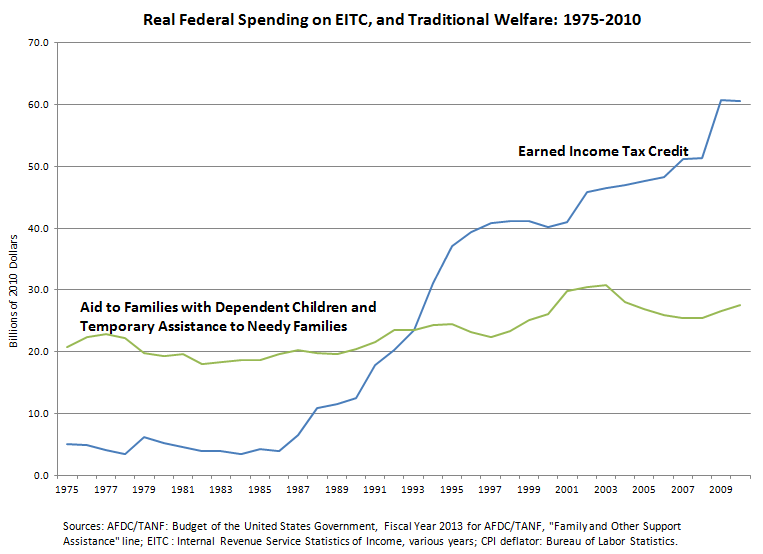
\includegraphics[width=0.9\textwidth]{graph.png}
\end{figure}

Even though tax expenditure spending should be viewed analogously to visible government spending, the politics between the two types of policy are often times quite different and reactive to one another in a way not previously outlined in the literature. One illustrative example is the case of poverty in America. Building on a state run program to aid single mothers, Congress passed a program called Aid to Dependent Children (ADC) which subsidized those state programs for that constituency. By the 1960s, through a series of eligibility changes enacted over the previous thirty years, ADC was the biggest welfare program in the country and served many more types of constituencies than just single mothers. As more Americans became eligible and started receiving ADC, it became increasingly unpopular among the public and elites. Even though the program had never been popular among Americans, it was especially vulnerable to retrenchment in the early years of the Nixon presidency. With the main poverty alleviation program unlikely to be expanded, but with the problem of poverty remaining, elites still wished to legislate around the issue. In 1974 and in spite of the desperately unpopular AFDC\footnote{The program was renamed from Aid to Dependent Children to Aid to Families with Dependent Children during the Great Society.}, Congress quietly passed a refundable tax credit for the working poor. The Earned Income Tax Credit (EITC) as it was called was a wage subsidy for low income people that would zero out their income tax liability and if any of the reward remained, the federal government would send the recipient a check for the remainder. While ADC was never expanded again and ultimately repealed and replaced with a far different program, the Earned Income Credit, social policy through the tax code, was expanded both in eligibility and generosity several times in subsequent decades \citep{stewart1991}. This is clearly seen in the above graph where the EITC explodes in cost relative to AFDC and AFDC remains basically stagnant once the EITC is introduced. The relationship between hidden and visible programs has not been  explicitly discussed in the literature yet we have much to learn from this sort of policy relationship. Why did legislators abandon expansions of ``visible'' welfare spending? Why was there a steady uptick in hidden spending even though it did almost the same thing as the now stagnant visible spending? Ultimately, we do not know why these seemingly similar programs have had such different historical trajectories with AFDC being abolished in 1995 when the EITC, which cost nearly twice as much as AFDC, was left totally untouched and is still used today. \citep{myles1997}.

In any case, American social policy uses four different types of mechanisms that both work together and compete with one another to provide services. Over time, these services and policies layer upon one another because political contexts change, which open or close different policy streams, changing the relative effectiveness and impact of the tools used to create policy \citep{kingdon2011}. Sometimes policies are retrenched and removed like in the case of ADC and sometimes the policies surrounding some issue grow and grow because other avenues are closed off like in the case of the EITC. Additionally, that different tools create different types of policies (even though they may serve the same goal), creates different politics. As illustrated above, the politics of visible programs may be radically different from the politics of tax expenditure programs. All of these factors come together to form the `exceptional' American welfare state -- a disparate web of interconnected and sometimes competing policies which have layered over time and have been enacted through one of four distinct policy making mechanisms.

With that in mind, this dissertation deals solely with the spending part of the equation, that is visible and hidden spending. The hidden welfare state literature has not been sufficiently linked with the extremely well developed research on the visible welfare state and this dissertation seeks to construct such a link. Ultimately, the conventional wisdom as it pertains to the hidden welfare state deals almost entirely with hidden \emph{spending} and analyzing hidden spending vis-a-vie visible spending drastically increases our knowledge over the spending part the American welfare regime. In any case, future research will need to keep broadening the scope while discussing explanations for the exceptional American welfare state to include rights and regulation and while they are important in general, they are not important to this story.

\subsection{Why does American social policy look this way?}
Having briefly described the mechanisms that the government uses to produce American social policy, we now turn to an overview of why and how the United States created and maintains this type of welfare regime. The United States has a fragmented welfare state with several different types of policies for each goal it tries to alleviate. How did America reach that point? Most research on the American welfare state deals with hypotheses for why the United States has limited \emph{visible} social spending when compared to other developed countries while at the same time, largely overlooking non visible aspects of the welfare system. 

While imperfect, the explanations for the lack of visible social spending in the United States are a good start for discussing policy making overall. Political science does not understand very well what factors lead politicians to utilize one policy making tool over another in either the creation process or the maintenance process. In other words, the conventional theories are static in outlook and are unable to explain why one type of welfare spending increases while another decreases. Questions of visible spending are very much the conventional questions in American welfare state research. Pragmatically, by initially focusing on the conventional wisdom we can clearly draw out areas that are overlooked.

Some scholars think that the United States lacks visible spending because American elites and citizens do not want to have a `generous' welfare state \citep{king1973}. The scholars who make this sort of argument generally rely on terms such as political culture or public opinion data to argue that Americans do not believe in a Scandinavian style welfare system. As such, politicians do not feel the pressure to pass that style of welfare and supporting such programs might even be an overall negative for the politician. It is worth noting that support for current welfare programs is relatively high suggesting that American political culture is not a complete explanation for the relative lack of visible welfare spending \citep[Ch. 6]{howard2008}.

Other scholars argue that the relationship between labor, business and the state is responsible for variation in social spending \citep{korpi1980, swenson2004}. This argument, often times called the social democratic model or power resources theory, highlights how the interactions between capital, labor, and the state affected the welfare policy creation process. However, these hypotheses are not in full agreement as to the role of any of these actors. Some scholars emphasize that organized labor had to overcome `naturally hostile' business interests in order to expand welfare programs and that American labor was simply unable to do that. Others argue that large business interests worked with the federal government to create certain welfare programs to offload business expenses to the government. In any case, these scholars emphasize the role of business and unions (or lack thereof) to explain the creation (or lack thereof) of the American welfare state. 

The third major hypothesis is that the American institutional arrangements create a barrier to passing legislation in general and this drastically reduces the federal government's ability to create expansive welfare policies \citep{pierson1995, robertson2011}. One exceptionally American trait is that the United States has an extremely large number of spots along the policy making process where a proposal's journey can be derailed if a key person or group does not support the proposal. The multitude of veto points or veto players, as they are called, allows a large number of ways to stop legislation unless veto players are appeased in some way. This includes formal legislative points such as passing a proposal out of committee or overcoming a filibuster as well as less formal elements like interest group support. One prominent way which veto points limited visible spending in the United States is that southern Democrats delayed and reduced welfare spending during the New Deal period in order to ensure African Americans were not able to receive the same level of benefits as whites \citep{katznelson2013}. 

These three schools of thought, as I have said, only deal with visible spending as a `dependent variable.' Obviously one major problem with this approach is that it does not deal with hidden spending in any meaningful way. Further, social policy creation is occurring in a more incremental way in the United States in the less visible policy arenas. While these canonical theories may be able to explain the New Deal social legislation or the Great Society social legislation they are unable to explain how hidden policies gradually advanced over time. Additionally, they are unable to explain why the legislature adopted a hidden policy over a visible policy (or vice versa). Just within the spending category, a legislator may choose to advance his or her policy goals with either the more traditional visible spending or spending through tax expenditures.

One good way to deal with this problem is to view social policy as goal oriented rather than focusing on individual policies. The United States encourages housing in several ways, such as, by allowing home owners to deduct part of their mortgage from their income taxes, providing public housing, providing section eight housing vouchers, and several other policies. By focusing solely on one of these policies (or one type of policy) to the exclusion of the others, we cannot say that we understand how social policy is made in the United States. It is only through dealing with, in this case, housing policy as a whole that we will be able to better understand social policy making.

Another separate problem is that these theories are largely concerned with policy creation and not subsequent policy development. While policy creation is important, there are two constituent parts of American social policy -- creation and maintenance -- which need to be discussed in attempting to understand the policy making process. The lack of attention to what happens to policy \emph{after} enactment undermines our understanding of the policy making process as a whole especially when policy development can be just as important as policy enactment \citep{patashnik2008}. For instance, if we only concerned ourselves with the creation of Social Security, we would still see a program that excluded large chunks of the population, was largely not a universal program, and still had relatively weak benefits. It was only through post creation development where Social Security became the program we know today \citep{derthick1979}.

Why would the United States create a hidden program \emph{instead} of a visible program? Why has hidden social policy continued to grow while visible social policy has stagnated? The United States has created lots of hidden policies before, in between, and after, the explosion of visible programs in the 1930s and 1960s yet we do not know why elites utilized different legislative strategies \citep[Ch. 2]{howard2008}. We also do not know why those hidden programs have been consistently expanded over the 20th century. Additionally, many of the hidden programs created during the non big bang periods had the same goals as the visible programs created in those periods such as encouraging higher education, reducing poverty, or providing health insurance, but we consider individual programs in isolation from the others. It is an important oversight that most conventional research on American social policy does not account for different ways of providing the policy, instead focusing unilaterally on one of the four earlier mentioned mechanisms. If policy is, in a general sense, continually being made, then there is a very large hole in our understanding of American social policy creation because we cannot explain why one type of policy was adopted over another.

\section{The Question of Visible versus Hidden Spending}
With that in mind, this dissertation will argue that the creation of the hidden welfare state was largely facilitated by innovative legislators who wished to advance some policy goal, but wanted to avoid the politics of traditional welfare. Additionally, the growth of the hidden state was perpetuated and exacerbated because there was political and institutional pressure on lawmakers to find new, easier, ways to legislate. 

The logic of this proposition is relatively straight forward. The story of the post war American Congress is one of increasingly strict rules, more powerful centralized leadership, and more polarization \citep{rohde1991, binder2003}. Additionally, the mid 1970s saw the rise of a new brand of activist conservative who was more aggressive in attacking traditional style welfare programs like AFDC and who wished to lower tax rates \citep{hacker2007}. The interaction of these two forces manifested itself in an increasingly hostile environment for social policy. Any potential demand for federal assistance did not dissipate just because of this hostile environment however and many legislators still wanted to advance more expansive social policies. For a select few legislators, they found that they were able to quietly get a tax expenditure passed -- often times by attaching it to a much bigger tax bill -- which then de facto increased social spending. That story applies to expansion as well as creation, but in more dramatic style. As the same forces which encouraged hidden policy making originally intensify, the same legislators and others simply want to keep advancing their social policy goals and the tax expenditure route implicit in the hidden welfare state became increasingly the path of least resistance. 

In this section, I hope to outline some of the forces which specifically influenced the creation and expansion of the hidden welfare state. First, I outline a series of changes in the way congressional rules and behaviors changed over the last fifty years which made passing legislation more difficult and encouraged new ways of policy making. Second, I outline how the rise of modern activist conservatism and how a new style of conservative learned to use activist government for their own means.

As I have already implied, one of the most important factors in creating and the expanding the hidden welfare state is the centralization of power in chamber leadership in the House of Representatives. Democrats in the mid 1970s wished to ``make the people who held positions of power responsible to rank and file Democrats" \citep[pg. 26, quote spoken by Rep. Donald Fraser (D-MN)]{rohde1991}. In pursuing this goal, Democrats instituted several intra-party reforms which drastically increased the power of centralized leadership. They stripped many powers from committee chairs and had them run for intra-party election to keep their chair. Additionally, many of the powers taken from the committees were placed within central party leadership. The logic behind the internal reforms they took was to empower the Democratic caucus as a whole and to remove the fiefdoms of deeply entrenched committee chairs. Instead of southern Democrats with lots of seniority setting the agenda, the caucus as a whole got to choose which policies would be advanced in a given Congress. By the 1980s, however, the caucus was empowering House leadership to negotiate policy on their behalf instead of merely acting as the agent of the party's majority \citep{sinclair1983, palazzolo1992, sinclair1998}

The effects of moving from a committee based House of Representatives to centralized leadership empowered by the party as a whole had on visible policy making were profound. Previously powerful individuals were now unable to exert their previously significant clout to advance their own policy goals. More importantly, the caucus became an active veto point on individual member policy goals when it pertains to traditional policies. If policies needed to be supported by the majority of the caucus to have any real possibility of being passed then members with goals in tension with the party faced a real challenge. Moving past the ideological issues, a legislative session has a limited amount of agenda space and time so even if a proposed policy was acceptable to the caucus it still might not be advanced because other things are more important.

These House chamber reforms were largely adopted by the Republicans when they won control of both chambers in 1994. With the movement from a committee centric Congress to a speaker centric Congress, conservatives in Congress were able to use the reforms passed by liberal Democrats in the 1970s to their own advantage as well \citep{zelizer2007}. Those with an interest in social policy now faced an even more hostile set of veto points because conservatives controlled the chamber and were actively trying to cut welfare spending. In the New Deal period and prior to the 1970s reforms more generally, the decentralized nature of the House chamber and the lack of well sorted congressional parties encouraged bipartisan and ideologically diverse voting coalitions \citep{poole1997}. This allowed even minority party members to realistically pursue their policy goals. The Republicans swept into office viewed themselves as ideological purists and were largely unwilling to compromise with the now minority Democrats \citep{hacker2006}. Combined with the largely centralized chamber power, Republicans were able to simultaneously pass large parts of the Contract with America and also discourage legislators who may have wanted to temper any welfare cuts \citep{aldrich2000}. 

In the Senate, the story is very much the same except it was the reciprocal norm of respect eroding \emph{alongside} an empowerment of chamber leadership \citep{sinclair1986}. Since the early 1980s individual senators have spent more resources empowering their party's leadership and those leaders changing the Senate agenda to maximize inter-party cleavages while minimizing their own party's ideological differences \citep{lee2008}. An obvious consequence of this type of agenda control is that it encouraged ideological sorting among Senators to the point where all conservatives were in one party and all liberals in the other. It was already difficult to pass legislation through the Senate due to supermajority requirements, so as parties became more homogenized the cost of moving the status quo increased \citep{koger2010}. Like in the House, a costly legislative process encourages members to develop new ways to legislative -- namely, through the tax code.

Outside of individual chambers of Congress, divided government also makes legislating difficult. Prominently, \cite{mayhew1990} argues that divided government has no real effect on `major' legislation passed in a given Congress. In this case, major legislation means highly salient legislation and by definition does not account for hidden spending. Conversely, divided government has been mentioned as relevant to the creation of hidden welfare spending. \citet[Ch. 4]{howard2008} argues that divided government is associated with more hidden welfare policies being made as it is harder to pass visible legislation in a divided government situation. Since 1970, the United States has had unified government 30\% of the time compared to 70\% for the earlier part of the 20th century. Again, as it becomes harder to pass legislation legislators need to find more innovative ways to advance their policy goals.

These are big changes in the American Congress which, I propose, go hand in hand with creation and expansion of the hidden welfare state at the expense of the visible welfare state. Over the last forty years, legislation has become increasingly more difficult to pass through Congress. Through a rise of restrictive rules, centralized chamber leadership, increased obstruction, and increased polarization, passing traditional social policy through the traditional policy making process became too costly for politicians. Legislators who still wanted to advance social policy needed to find other ways to achieve their goals. By making policy through the tax code, legislators found a tool that did not require as much political capital to advance and was not even on the radar of most other members of Congress. By using the tax code, legislators constructed the hidden welfare state by carving out exemptions and constructing expenditures which allowed them to reward certain behavior without most other MCs realizing what was happening. 

As Congress was changing, so to was American conservatism. The rise of the modern American conservative movement came directly as a reaction to the New Deal and the Great Society, and the activist state more generally \citep{critchlow2007, zelizer2010}. They resented taxation in general and using the money to fund a welfare state was deeply unpopular. In post war America, the overall conflict between liberals and conservatives was over the scope and size of the federal government. Conservatives wished to retrench New Deal and Great Society programs and generally wanted the federal government to do less. The nature and tactics of conservatives started to change in late 1960s though with an increase of conservatives wishing to use the government to pursue their own policy goals instead of just stopping activist government \citep{teles2007, skocpol2007}. To that end, conservatives, began to use the levers of activist government created by liberals to pursue their own policy goals \citep{hacker2004}. This new style of conservatism exacerbated the growth of the hidden welfare state as many of the newer activist style conservatives learned they could advance a policy goal and also say they were cutting taxes.

The evolution and rise of modern conservatism combined with the changes of congressional behavior and rules, I propose, can largely explain the creation and expansion of the hidden welfare state. As Congress changed so did the policy it produced. Similarly, as the ideological and tactical inputs of conservatives changed, so did policy. Consequently, politicians deliberately choose less visible policy making techniques because it is easier for those policies to pass and also become entrenched. Like with the visible welfare state, related policies layer on one another, resulting in the fragmented welfare state that we have. Hidden and visible policies work in tandem in providing the American social safety net. More generally, public policy is created over time and is very tightly linked with the institutional arrangements that approve, develop, and administer the program \citep{pierson2004b}. The types of policies that are passed depend on the institutional constraints that the political actors are behaving under and the policy preferences of the actors themselves. By examining the rules and actors involved with a political process -- in this case the creation and development of the American welfare state -- we can illuminate the policy making process, American public policy, and the way political actors and political institutions interact.

 
\section{Research Design}
%\citep{elving1996}




\newpage
    \bibliography{EITC}{}
\bibliographystyle{jpe}

%\printbibliography
\end{document}


